%04.rancangan
\chapter{RANCANGAN BASIS DATA}

Rancangan struktur basis data akan terdiri dari beberapa tabel seperti berikut :

\section{Tabel SPPT}

Tabel ini selain mencatatkan ketetapan untuk tiap objek pajak pada tiap tahun pajak, tabel ini juga mencatatkan status pembayaran apakah sudah lunas atau belum pada kolom / \textit{field} \texttt{status\_pembayaran\_sppt}. Struktur tabelnya adalah seperti pada gambar \ref{fig:tab-sppt} berikut ini :

\begin{figure}[H]
	\centering
	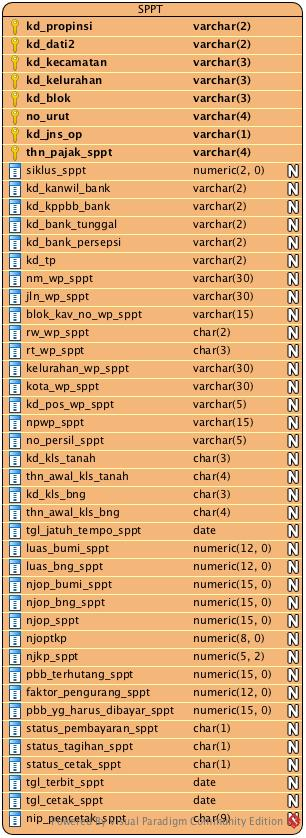
\includegraphics[width=0.5\textwidth]{./resources/struktur-tabel-sppt}
	\caption{Struktur Tabel SPPT}
	\label{fig:tab-sppt}
\end{figure}

Kolom atau \textit{field} yang dimanfaatkan dari tabel ini hanya beberapa bagian saja, yaitu :

\begin{itemize}
	\item Nomor Objek Pajak (NOP), yang terdiri dari \textit{field} atau kolom \texttt{kd\_propinsi}, \texttt{kd\_dati2}, \texttt{kd\_kecamatan}, \texttt{kd\_kelurahan}, \texttt{kd\_blok}, \texttt{no\_urut}, dan \texttt{kd\_jns\_op}.
	\item Tahun pajak pada \textit{field} atau kolom \texttt{thn\_pajak\_sppt}.
	\item Nama wajib pajak pada \textit{field} atau kolom \texttt{nm\_wp\_sppt}
	\item Besarnya pajak terhutang pada \textit{field} atau kolom \texttt{pbb\_yg\_harus\_dibayar\_sppt}
	\item Status pembayaran pada \textit{field} atau kolom \texttt{status\_pembayaran\_sppt}
\end{itemize}

\section{Tabel DAT\_OBJEK\_PAJAK}

Tabel \texttt{DAT\_OBJEK\_PAJAK}, digunakan untuk menampilkan informasi mengenai objek pajak seperti alamat, luas bumi dan bangunan, serta Nilai Jual Objek Bumi dan Bangunan. Struktur tabel dari \texttt{DAT\_OBJEK\_PAJAK} adalah seperti pada gambar \ref{fig:tab-dat-op} berikut ini :

\begin{figure}[H]	
	\centering
	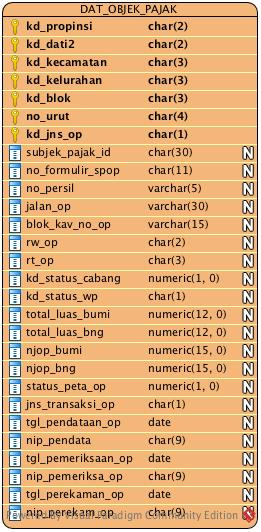
\includegraphics[width=0.3\textwidth]{./resources/struktur-tabel-dat-op}
	\caption{Struktur Tabel \texttt{DAT\_OBJEK\_PAJAK}}
	\label{fig:tab-dat-op}
\end{figure}

\section{Tabel DAT\_SUBJEK\_PAJAK}

Tabel \texttt{DAT\_SUBJEK\_PAJAK} ini digunakan untuk menampilkan informasi mengenai subjek pajaknya seperti nama dan alamatnya. Struktur tabel dari \texttt{DAT\_SUBJEK\_PAJAK} ini adalah seperti pada gambar \ref{fig:tab-dat-sp} berikut ini :

\begin{figure}[H]
	\centering
	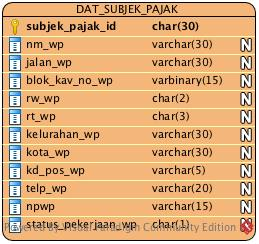
\includegraphics[width=0.3\textwidth]{./resources/struktur-tabel-dat-sp}
	\caption{Struktur Tabel \texttt{DAT\_SUBJEK\_PAJAK}}
	\label{fig:tab-dat-sp}
\end{figure}

\section{Tabel REF\_KECAMATAN}

Untuk tabel \texttt{REF\_KECAMATAN} digunakan hanya untuk menampilkan informasi nama Kecamatan dimana objek berada. Struktur tabel untuk \texttt{REF\_KECAMATAN} ini seperti terlihat pada gambar \ref{fig:tab-ref-kec} berikut ini :

\begin{figure}[H]
	\centering
	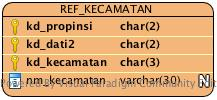
\includegraphics[width=0.3\textwidth]{./resources/struktur-tabel-ref-kec}
	\caption{Struktur Tabel \texttt{REF\_KECAMATAN}}
	\label{fig:tab-ref-kec}
\end{figure}

\section{Tabel REF\_KELURAHAN}

Tabel \texttt{REF\_KELURAHAN} pun digunakan hanya untuk menampilkan nama Kelurahan / Desa dimana objek pajak berada. Struktur tabel \texttt{REF\_KELURAHAN} ini seperti terlihat pada gambar \ref{fig:tab-ref-kel} berikut ini :

\begin{figure}[H]
	\centering
	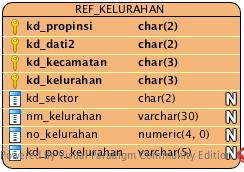
\includegraphics[width=0.3\textwidth]{./resources/struktur-tabel-ref-kel}
	\caption{Struktur Tabel \texttt{REF\_KELURAHAN}}
	\label{fig:tab-ref-kel}
\end{figure}

